\documentclass[a4paper, 12pt]{article}

\usepackage[T1]{fontenc}
\usepackage[utf8]{inputenc}
\usepackage[english]{babel}  % ngerman for German
\usepackage{lmodern}  % nicer font
\usepackage{geometry}
\geometry{%
	left   = 2.5cm,
	right  = 2.5cm,
	top    = 3cm,
	bottom = 3cm
}

\usepackage{textcomp}
\usepackage{gensymb}
\usepackage{amsmath,amssymb,amsfonts}
\usepackage{nicefrac}  % nicer inline fractions
\usepackage{tensor}  % allows fancy indices
\usepackage{siunitx}  % easy handling of value + unit (e.g. \SI{10}{\pF})
% \sisetup{}  % configure siunitx (e.g. locale = DE)
\sisetup{output-complex-root=\ensuremath{\mathrm{j}}, complex-root-position = before-number} % configures SI format 10 + j5 for complex numbers (instead of 10 + 5i)

\usepackage{listings}  % code listings
\usepackage{enumerate}
\usepackage{booktabs}  % nicer tables (e.g. \toprule)
\usepackage{verbatim}  % inline code (\verb||)
\usepackage{subcaption}  % captions for subplots
\usepackage[european, siunitx, RPvoltages]{circuitikz}  % draw circuit diagrams
\usepackage{enumitem}
\setlist[itemize]{label=\rule[0.5ex]{0.6ex}{0.6ex}} % black squares for itemize

\usepackage{pstool}  %% Tex fonts in EPS files
\usepackage{graphicx}
\graphicspath{{./figures/}}

\usepackage{etoolbox} % Needed for AtBeginEnvironment command (appendix handling)
\usepackage{appendix} % Appendices environment

\usepackage{csquotes} % removes biber warning
\usepackage[  % ieee style citations (e.g. [1])
	backend     = biber,
	maxbibnames = 99,
	autocite    = footnote,
	style	    = ieee,
	citestyle   = numeric-comp,
	doi=false, isbn=false
]{biblatex}
\addbibresource{bibliography/bibliography.bib}

\usepackage[nobiblatex]{xurl}  % line breaks in URLs
% last imports
\usepackage[bookmarksopen,colorlinks,citecolor=black,linkcolor=black, urlcolor = black]{hyperref}

% after hyperref! 
\usepackage[noabbrev, nameinlink]{cleveref} 
% e.g. \cref{label} or \Cref(label) for capital letter
% configure cleveref not to use brackets around equation references
\creflabelformat{equation}{#2\textup{#1}#3} % Equation references without parentheses
\AtBeginEnvironment{appendices}{\crefalias{section}{appendix}} % Appendix referencing (for cref "Appendix A" instead of "Section A")


% add missing hyphenations
\hyphenation{im-ple-men-ta-tions}

\title{ECS7012P - Music and Audio Programming\\
	   Assignment 1: Synth Filter}
\author{
  Max Tamussino, 200579179
}
\date{\today}


\begin{document}

\maketitle
\tableofcontents
\pagebreak

\section{Introduction} \label{sec:intro}
This report discusses the implementation of a digital emulation \cite{Stilson1996} of a Moog voltage-controlled filter \cite{Moog1965}. The overall structure of this filter is depicted in \Cref{fig:overall-structure}. It consists out of four first-order low-pass filters, a simple nonlinear function and a feedback loop.

\begin{figure}[h!]
	\centering
	\includegraphics[width=0.9\textwidth]{feedback.jpg}
	\caption{Overall structure of the implemented Moog voltage-controlled filter, adapted from \cite{Vaelimaeki2006}}
	\label{fig:overall-structure}
\end{figure}

\section{First-order filter section} \label{sec:first-order-fs}
\subsection{Derivation}
As proposed in \cite{Vaelimaeki2006}, one of the four first-order sections of the filter is implemented as depicted in \Cref{fig:first-order-section}. The equations for the individual nodes annotated are given in \Cref{eq:nodes1,eq:nodes2,eq:nodes3,eq:nodes4}. 

\begin{align}
	\label{eq:nodes1}
	A &= \frac{1}{1.3} \cdot x[n] & B &= x[n-1] \\
	\label{eq:nodes2}
	C &= \frac{0.3}{1.3} \cdot B & D &= A + C \\
	\label{eq:nodes3}
	E &= y[n-1] & F &= D - E \\
	\label{eq:nodes4}
	G &= g \cdot F & y[n] &= E + G
\end{align}

The filter equation given in  \Cref{eq:filter} was then derived from these equations.

\begin{equation}
	\label{eq:filter}
	y[n] = g \frac{1}{1.3} \cdot x[n] +
	g \frac{0.3}{1.3} \cdot x[n-1] +
	(1-g) \cdot y[n-1]
\end{equation}

The filter equation was then compared to the standard form of a first-order IIR filter, which is given in \Cref{eq:first-order-iir}.

\begin{equation}
	\label{eq:first-order-iir}
	y[n] = b_0 \cdot x[n] + 
	b_1 \cdot x[n-1] - 
	a_1 \cdot y[n-1]
\end{equation}

The resulting filter coefficients $b_0$, $b_1$ and $a_1$ were then calculated and are given in \Cref{eq:coefficients}.

\begin{align}
	\label{eq:coefficients}
	b_0 &= g \frac{1}{1.3} &
	b_1 &= g \frac{0.3}{1.3} &
	a_1 &= g - 1
\end{align}

\begin{figure}
	\centering
	\includegraphics[width=0.8\textwidth]{first-order-section.jpg}
	\caption{First-order section of the filter depicted in \Cref{fig:overall-structure}, adapted from \cite{Vaelimaeki2006}}
	\label{fig:first-order-section}
\end{figure}

\subsection{Performance}

The parameter $g$ of the filter coefficients is firstly calculated simply by $g = 2 \pi \cdot f_c / f_s$. The filter frequency response using this formula is given in \Cref{fig:prim-resp} for the two different cutoff frequencies. It is clearly visible that the intended cutoff frequencies were not met accurately. In \Cref{fig:prim-resp}, for $f_c = \SI{1}{\kilo\hertz}$, the response shows its cutoff at approximately \SI{1.1}{\kilo\hertz}, resulting in an error of \SI{10}{\percent}. For $f_c = \SI{4}{\kilo\hertz}$, \Cref{fig:prim-resp} even shows its cutoff frequency at approximately \SI{5.57}{\kilo\hertz} - an error of \SI{39.3}{\percent}.

To mitigate the nonlinear relation of $f_c$ to the actual cutoff frequency, a polynomial model for the parameter $g$ is proposed in \cite{Vaelimaeki2006}. The model is given in \Cref{eq:polynom-fit}, where $\omega_c = 2 \pi \cdot f_c / f_s$. The result for the frequency response of the filter is given in \Cref{fig:ext-resp}. For $f_c = \SI{1}{\kilo\hertz}$, the error was reduced to \SI{2}{\percent} (actual cutoff \SI{1.02}{\kilo\hertz}). For $f_c = \SI{4}{\kilo\hertz}$, the real cutoff frequency is around \SI{4.12}{\kilo\hertz}, a significantly improved error of only \SI{3}{\percent}.

\begin{equation}
	\label{eq:polynom-fit}
	g = 0.9892 \omega_c - 0.4342 \omega_c^2 + 0.1381 \omega_c^3 - 0.0202 \omega_c^4
\end{equation}

\begin{figure} [!h]
	\centering
	\begin{subfigure}[b]{0.9\textwidth}
		\centering
		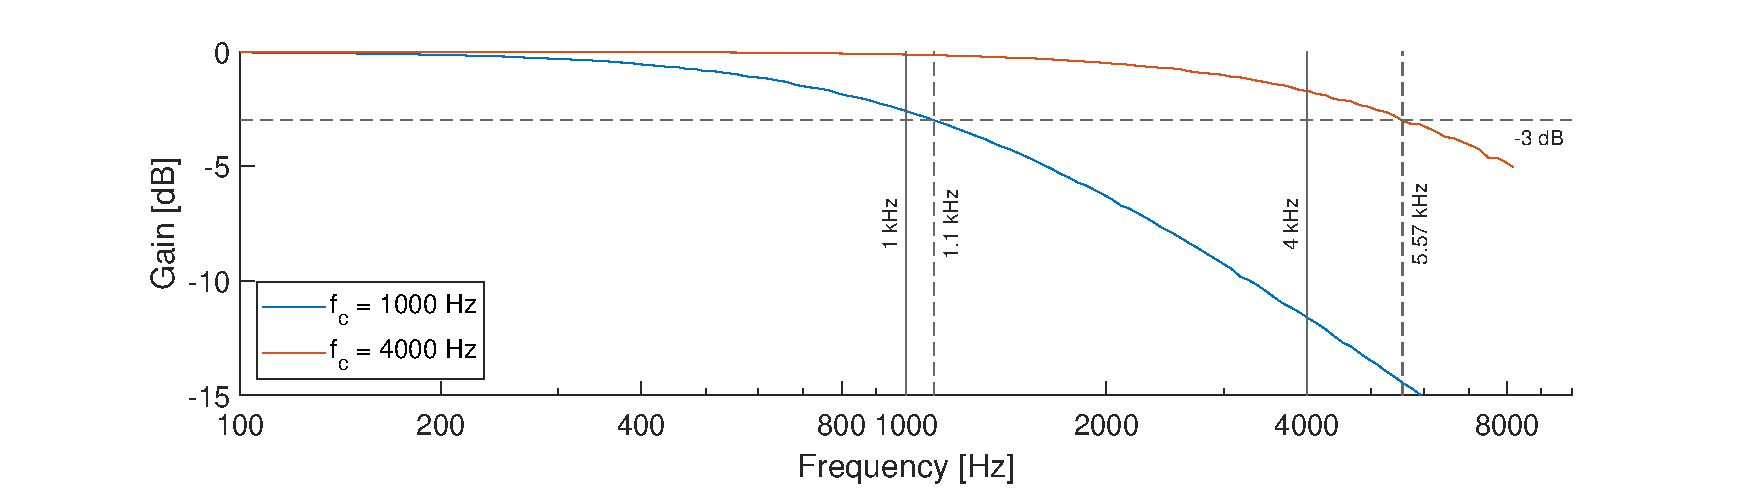
\includegraphics[width=\textwidth]{primitive-responses.eps}
		\subcaption{Primitive calculation ($g = 2 \pi \cdot f_c / f_s$)}
		\label{fig:prim-resp}
	\end{subfigure}
	\begin{subfigure}[b]{0.9\textwidth}
		\centering
		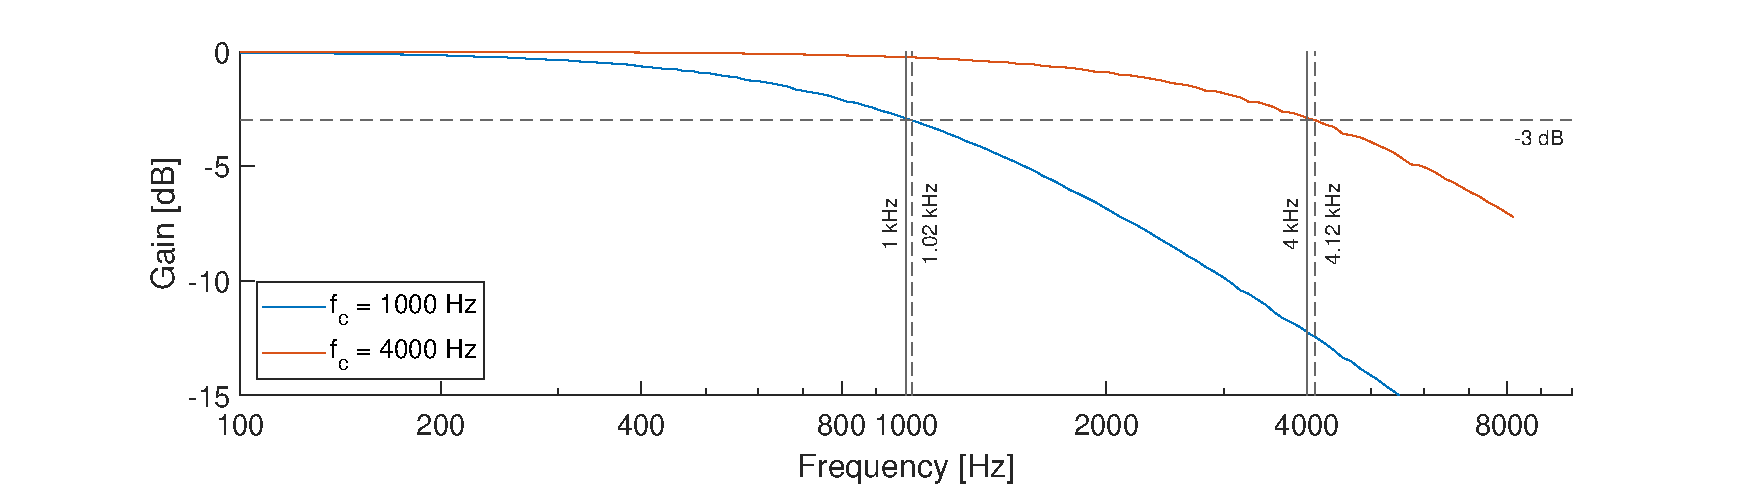
\includegraphics[width=\textwidth]{improved-responses.eps}
		\subcaption{Polynomial fit (see \Cref{eq:polynom-fit})}
		\label{fig:ext-resp}
	\end{subfigure}
	\caption{Filter responses for different calculations of parameter $g$}
	\label{fig:g-resp}
\end{figure}

\section{Fourth-order filter} \label{sec:fourth-order}
The combination of four first-order filter segments (discussed in \Cref{sec:first-order-fs}) results in a fourth-order filter. The frequency response of this combination is given in \Cref{fig:fourth-order-resp}. At the \SI{-3}{\deci\bel}-frequency of the first-order section, the fourth-order response shows a gain of \SI{-12}{\deci\bel}. This is expected, as four identical filter elements with \SI{-3}{\deci\bel} gain are combined.

\begin{figure}[!h]
	\centering
	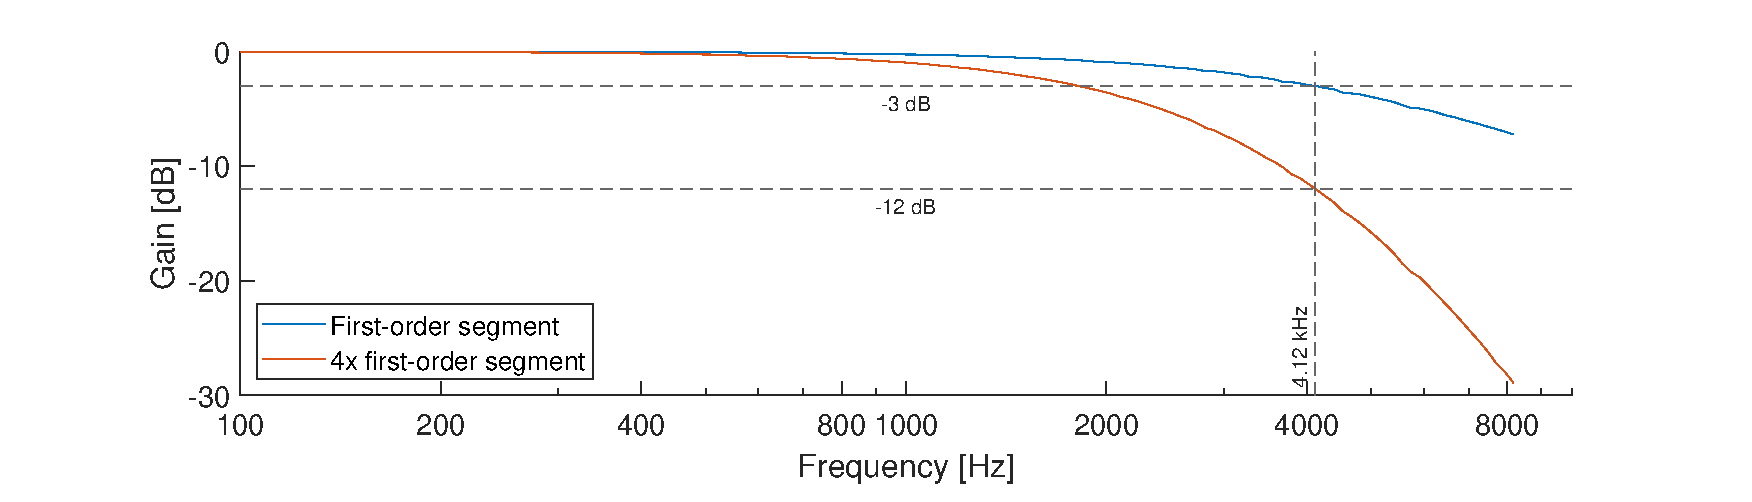
\includegraphics[width=0.9\textwidth]{fourthorder-response.eps}
	\caption{Filter response for four of the first-order sections combined, each using $f_c = \SI{4}{\kilo\hertz}$}
	\label{fig:fourth-order-resp}
\end{figure}

\section{Nonlinearity}
The nonlinear function $\tanh(x)$ is applied \cite{Huovilainen2004} to the input before filtering, which is depicted in \Cref{fig:overall-structure}. This introduces signal distrotion. Especially for high amplitudes, the peaks of input sine waves are flattened. In the frequency domain, this effect introduces additional harmonics which increase in significance for high input amplitudes. For low amplitudes however, no significant harmonics are introduced. This is due to the shape of the function $\tanh(x)$, which is very close to being linear for low and increasingly nonlinear for high input amplitudes.

\section{Feedback}
The feedback path depicted in \Cref{fig:overall-structure} requires transformation into an equation. Therefore, the equations for the nodes annotated are derived in \Cref{eq:nodes5,eq:nodes6,eq:nodes7}. For the implementation, the parameter $G_{comp}$ is set to a fixed value of $0.5$. An example response for $G_{res}=0.75$ is shown in \Cref{fig:feedback-response}. It shows a resonant peak at \SI{870}{\hertz} with a maximum gain of \SI{7.2}{\deci\bel}.

\begin{align}
	\label{eq:nodes5}
	J &= y[n-1] & K &= G_{comp} \cdot x[n] \\
	\label{eq:nodes6}
	L &= J - K & M &= 4 G_{res} \cdot L
\end{align}
	
\begin{equation}
	\label{eq:nodes7}
	N = x[n] - M = x[n] - 4 G_{res} \cdot (y[n-1] - G_{comp} \cdot x[n])
\end{equation}

\begin{figure}
	\centering
	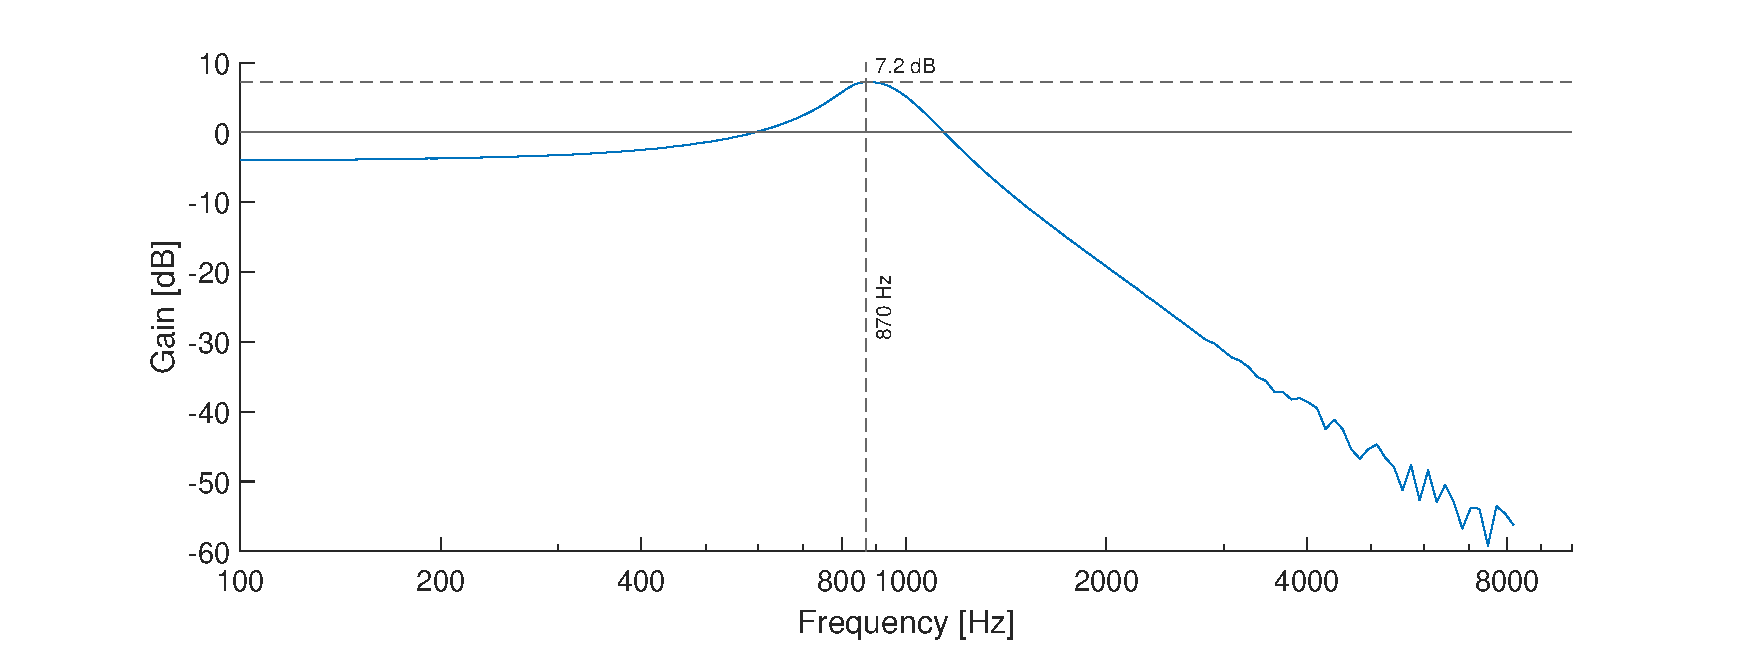
\includegraphics[width=0.9\textwidth]{feedback-response.eps}
	\caption{Filter system frequency response using feedback, first-order segments with $f_c = \SI{1}{\kilo\hertz}$ and $G_{res}=0.75$}
	\label{fig:feedback-response}
\end{figure}

\section{Adjustable resonance}
Using the parameter $C_{res} \in [0, 1]$, the resonance peak can be adjusted by using \Cref{eq:gres-polynom} for $G_{res}$ \cite{Vaelimaeki2006}. The resonance frequency can simply be adjusted by re-calculating the first-order filter segments coefficients for a different cutoff frequency. The influence of this parameter is observed in \Cref{subsec:c-adjust}.

\begin{equation}
	\label{eq:gres-polynom}
	G_{res} = C_{res} \cdot (1.0029 + 0.0526 \omega_c - 0.0926 \omega_c^2 - 0.0218 \omega_c^3)
\end{equation}

\section{Experiments}
\subsection{Effect on sawtooth spectrum}
As a simple experiment, a sawtooth oscillator with frequency $f=\SI{100}{\hertz}$ and amplitude $A=0.3$ was used as an input to the implemented system (using $C_{res}=0.9$ and $f_c = \SI{2}{\kilo\hertz}$). \Cref{fig:fft-sawtooth-resonance} shows the Fast Fourier Transformation (FFT) of this input and the resulting output. The resonant peak is clearly visible at approximately \SI{2}{\kilo\hertz}. Changing the resonance frequency is furthermore clearly audible, as this specific frequency of the sawtooths spectrum is especially amplified.

\begin{figure}[h!]
	\centering
	\includegraphics[width=0.7\textwidth]{fft-sawtooth-resonance.jpg}
	\caption{FFT of sawtooth oscillator input with $f=\SI{100}{\hertz}$ and amplitude $A=0.3$ (red) and the resulting output using $C_{res}=0.9$ and $f_c = \SI{2}{\kilo\hertz}$ (blue)}
	\label{fig:fft-sawtooth-resonance}
\end{figure}

\subsection{Sudden input removal}
This experiment uses the same setting as before, only the resonance parameter was maximised to $C_{res}=1$. After turning down the input oscillator amplitude to zero, the system output showed only its resonance frequency for approximately \SI{1}{\second}. The high gain at this frequency, combined with feeding back the output to the filters input, results in this behaviour.

\subsection{Resonance adjustment} \label{subsec:c-adjust}
In the final experiment, a bode plot of the complete system is made for five different values of $C_{res}$. The filter cutoff frequency is set to $f_c = \SI{1}{\kilo\hertz}$. The results are depicted in \Cref{fig:c-adjust}. It is interesting that the parameter $C_{res}$ does not only influence the height of the resonance peak, but also the resonance frequency and the gain for low frequencies.

\begin{figure}[h!]
	\centering
	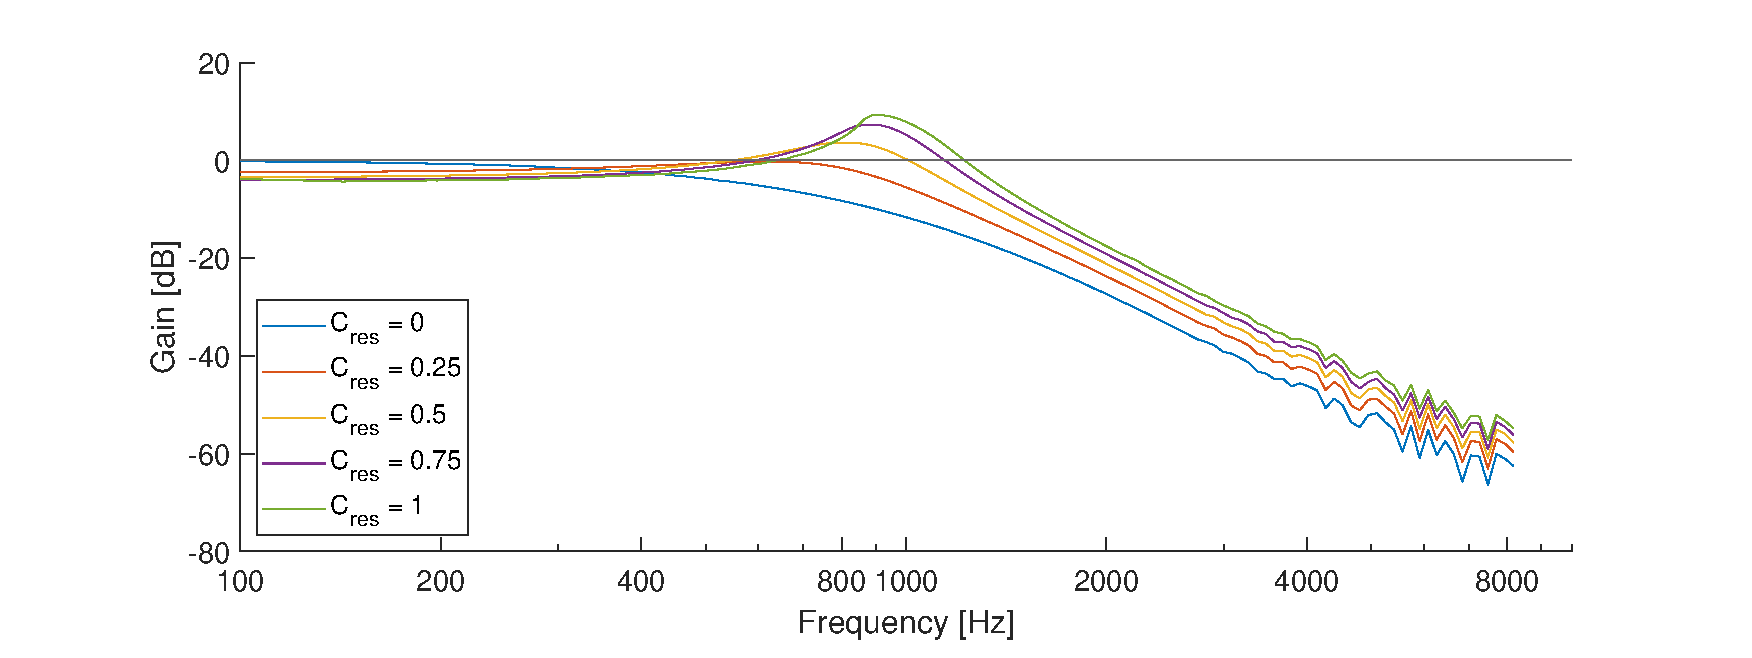
\includegraphics[width=\textwidth]{resonances.eps}
	\caption{Frequency response of filter system with $f_c = \SI{1}{\kilo\hertz}$ and different values for $C_{res}$}
	\label{fig:c-adjust}
\end{figure}

\sloppy
\printbibliography

\end{document}